
This doctoral dissertation studies the applicability of novel machine learning methods with remote sensing data in the context of agricultural decision support systems (DSS) in precision agriculture \cite{Bell1995} and smart farming \cite{Sundmaeker2016}. Farmers have practiced precision agriculture for ages to optimize yield productions of their fields. Sources of intra-field variability were deduced by noting and exchanging annual observations and experimenting with interventions. However, both the observations and the conclusions drawn have been more or less based on intuition, rather than on objective data. From this emerges the need for data-driven decision making, i.e. smart farming, to aid the farmers in choosing the best actions to take to optimize crop cultivation \cite{Kamilaris2017}. The application of novel deep learning techniques has been on an increasing trend for the past few years in smart farming and precision agriculture application domains \cite{VanKlompenburg2020}. One of the key reasons for this progression is the abundant availability of sensor based data in terms of ground-based soil sensors, and low-altitude unmanned aerial vehicles (UAV) and high-altitude satellite systems \cite{Wolfert2017d}. Another factor is the open-access availability of other enviromental data, such as weather and land survey data. Thus, the use of remote sensing data to extract information with machine learning models for data-driven decision making has become more common. Especially, the number of studies using deep learning techniques to perform agriculture related modelling tasks has steadily increased \cite{Kamilaris2018a}. 

Remote sensing data relevant to smart farming tends to be predominantly spatial in nature. This stems from the objects of interest - fields, forests and plots of land. Conventionally, open-access remote sensing data has been acquired from nationally operated multispectral satellite sources, such as Sentinel-2 (ESA, Paris, France) or Landsat 8 (USGS, Reston, Virginia, USA). Satellite data, while spatial, is also temporal due to regular and frequent overflights over land and sea surfaces. Commercially available UAVs have also been utilized \cite{Nasi2017}. While some UAVs come pre-fitted with quality RGB sensors, some systems are designed as platforms to which then desired sensor technology is to be mounted. Due to the altitude from which the data is acquired, satellite and UAV data differ greatly in spatial resolution. This is illustrated in Figure~\ref{fig:uav-s2-block}, where (a) is an orthomosaic of UAV iamges of a field and (b) is the corresponding image as captured by Sentinel-2 satellite at approximately the same time. While the pre-fitted RGB cameras of UAVs allow data capture resolutions well below 1 m/px, open-access satellite data is available at resolutions starting from 10 m/px (Sentinel-2). These data, satellite and UAV, are readily in image-like spatial format. Other field-related observational data, such as data from soil sensors or soil samplings, are often interpolated over plots of interest to generate image-like data in the form of spatial rasters. 

\begin{figure}[htb]
    \centering
    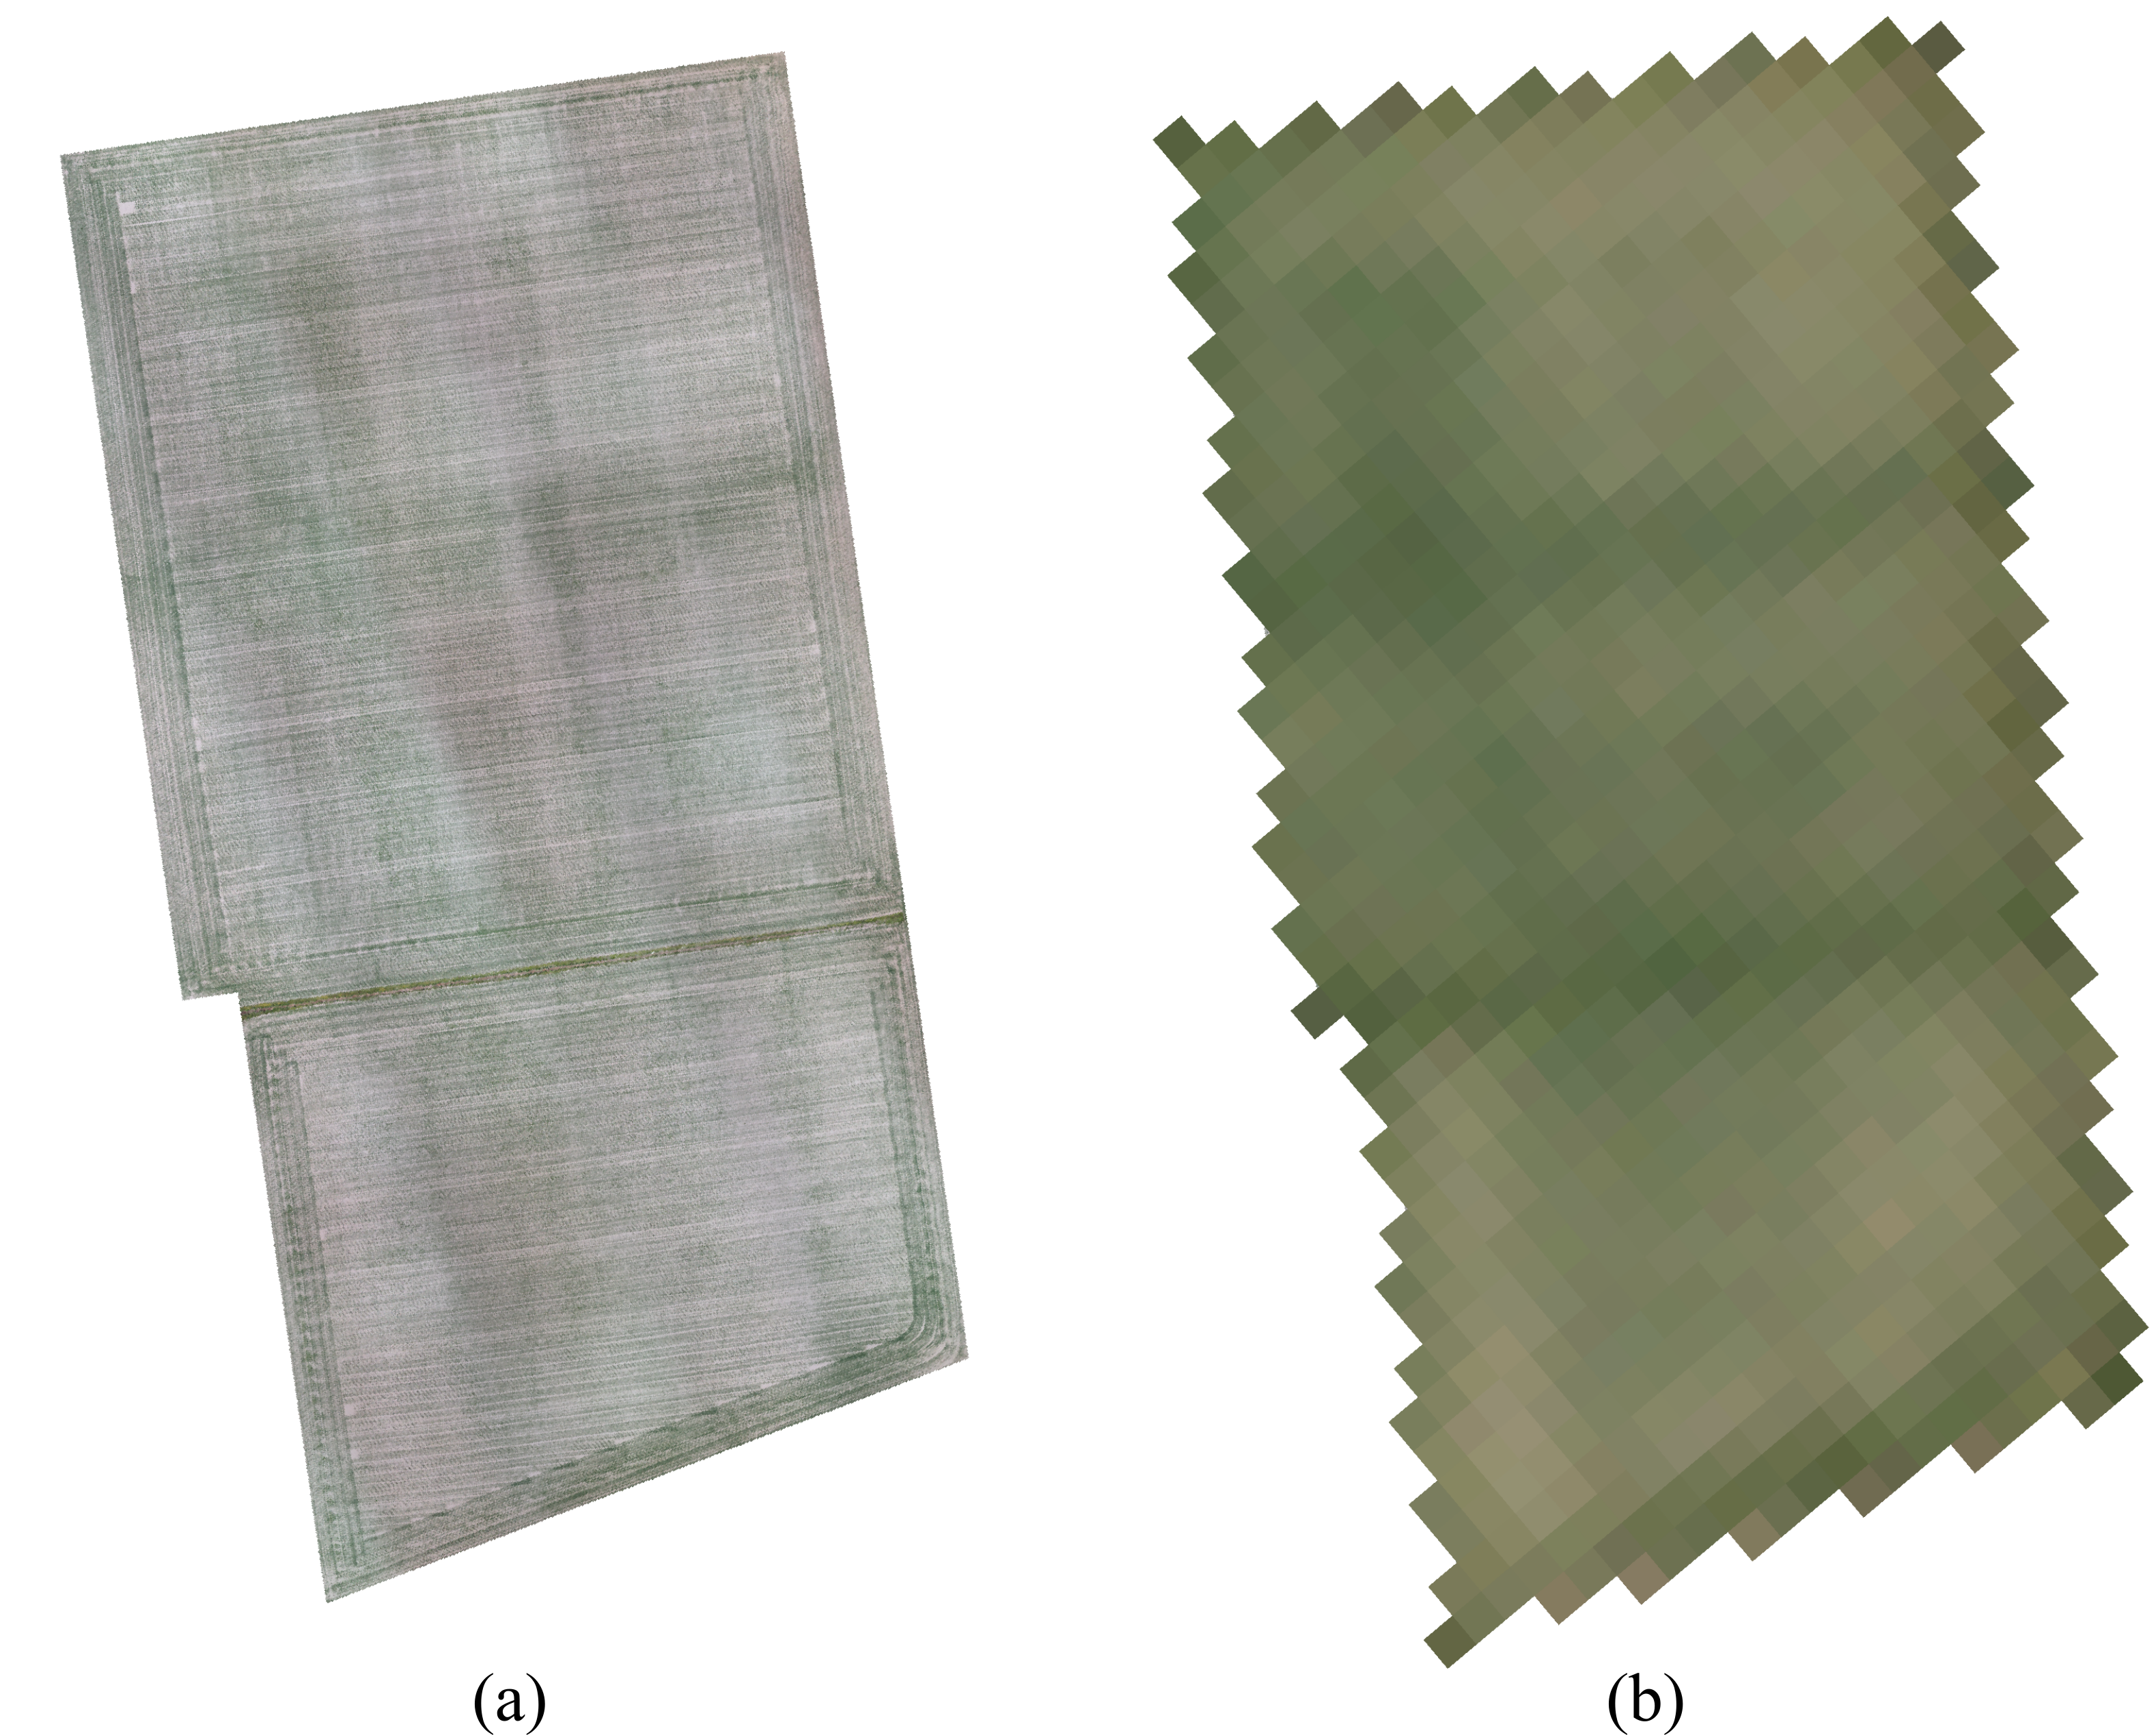
\includegraphics[width = \textwidth]{images/uav-s2-block.png}
    \caption{images of a field from week 24 of 2018 from (a) UAV and (b) Sentinel-2.}
    \label{fig:uav-s2-block}
\end{figure}

The form of input data directly effects the selection of suitable data-based modelling techniques. Convolutional neural networks (CNN) \cite{LeCun1989,LeCun1998b}, a subset of neural network based deep learning techniques, excel with spatial data related tasks. These tasks include object recognition, imgae classification and image-based regression. Recently, multiple studies have been conducted with CNNs in the context of agriculture and smart farming \cite{Kamilaris2018b}. The use of sequential models capable of extracting temporal features is also relevant with remote sensing data. Long short-term memory (LSTM) networks \cite{Hochreiter1997,Gers2000}, an implementation of recurrent neural networks (RNN) \cite{RumelhartDavidE1986Lrbb}, have been shown to perform well in modelling tasks involving sequential data \cite{Jozefowicz2015}. The LSTMs have to be coupled with CNNs to perform spatiotemporal modelling. Another way to tap into spatiotemporal data is to use three dimensional CNNs, where two dimensions are used for single point-in-time spatial inputs and the third dimension as the dimension of change between distinct spatial inputs \cite{Tran2015}. 

\section{Research questions}

In the context of using field related remotely and manually gathered data, the research questions of this study are:


\begin{itemize}
    \item[] \textbf{RQ1.} Can intra-field yield variability be reliably predicted using deep learning models based on high resolution remote sensing data from the early phase of the growth season?
    \item[] \textbf{RQ2.} Which data sources add value to high resolution yield prediction with deep learning models?
\end{itemize}

RQ1 is heavily centered around data based modelling with field related data. Excelling at complex decision making with fuzzy problems, humans are ill-equipped to derive causal and correlational relationships, whether linear or non-linear, from larger bodies of raw numerical data. Spatial data, such as RGB images of a field, consist of thousands of data points with multiple values associated to a single point. Spatial deep learning models, on the other hand, have been specifically developed to perform input-output mapping with spatial data. Due to the nature of these models, they require black-box optimization techniques to find the optimal combination of various hyperparameters. Hyperparameters are values, that have an effect on the training and the capabilities of the model. These values are, for example, the learning rate coefficient of the model's optimizing algorithm or the number of neurons, a calculation unit, within a layer of the layered deep learning architecture. Succsefully attaining the first objective requires also proper handling of input and target data samples. The data has to be both ingestable by the models, while the model's results have to be meaningful and interpretable by us humans. An additional key aspect is the usability of the models in commercial production environments. Having to do with usage and adoption, the usability of the models as a part of a bigger DSS has to be evaluated.

Generally, deep learning models benefit from feature-rich data. Being non-linear and layered models, they are optimized during training to find the most effective combinations of input and hidden features built from the input data to accomplish the performance goals. Data, however, incurs a resource cost on the modelling process. Firstly, the data acquisition has an effect on the overall feasibility of the modelling. UAV data, for example, requires manual operation in Finland due to legislation and regulations. Secondly, the contribution to model performance is not equal between distinct data sources. Yet another aspect of data is its quality, which itself might affect the general performance of the model and the system the model is used in. Thus, the data used in the modelling has to be evaluated both in terms of feasibility and usability (RQ2).

For years, the number of farmers has been on a decline in Finland. With rather static number of field plots, the farms get bigger and are thus in need of better farm and process management tools. Manual, semi-automated and automated data acquisition from various operational areas require data processing automation to provide actionable items in actionable time frame. Thus, this study is an attempt to answer the question whether data based modelling is beneficial for farm management and process optimization.

\section{Publications and author's contribution}

The publications selected for this dissertation fall into three categories. The first category is about novel intra-field crop yield prediction model development. Publications [I] and [IV] belong to this category. The second category is related to data evaluation assessment. The publications belonging to this category are [III] and [V]. The last category is about the context in which crop yield modelling is performed, decision support systems for agriculture. Publication [II] belongs to this last category. For the publications in the first and the second category, the author did the majority of the work. In these publications, the author alone was responsible for accumulating, preprocessing and preparing the data from various sources. The author carried out the work of developing, implementing and training the models presented in the publications. Model performance evaluation and comparison to the state-of-the-art research was also conducted by the author. In those publications the author did not partake, however, in manual data acquisition, such as operating the UAVs during the growing season. The author of this dissertation was also responsible for writing the majority of text in these publications. In the publication [II] category, the work of the author was utilized in the study. The model architecture, code and results of [I] were utilized as a case study in the report.

\subsection*{Intra-field crop yield prediction model [I] [IV]}

Performing crop yield predictions from RGB image data requires using models capable of ingesting spatial data and deriving salient features from them. 
% CNNs, being shift and space invariant artificial neural networks \cite{Zhang1990}, are best suited for this modelling task. While open-access satellite data has already been utilized in crop related modelling, such as crop type classification and yield prediction, intra-field scale prediction with smaller fields common to Nordic countries requires images with higher resolution than what is currently available from the open-access satellite systems. More specifically, fields with side dimensions in just hundreds of meters are ill-represented by 10 m/px resolution satellite sources for intra-field modelling. Due to CNNs requiring input data having constant spatial dimensions, regular smaller frames are extracted from images of irregularly shaped fields. 
As part of the Mikä Data project carried out in the Data Analytics and Optimization research group of the Pori unit of Tampere University, several fields were imaged during the growing seasons of 2017-2019. UAV-based orthomosaic images of crop fields have the data in a resolution high enough to allow for extracting image frames of fixed dimensions.  The images of these fields were used to train models to perform frame-based crop yield prediction with single point-in-time [I] as well as time series [IV] image data. Throughout this study, point-in-time is used as an expression to distinquish between temporally distinct inputs from temporal sequences of multiple inputs. 
% Extensive tuning of optimizer related hyperparameters and architectural parameters is performed to find the best performing model composition in both modelling cases. 
The point-in-time model is based on a CNN, with its depth and configuration tuned to perform mapping of RGB image frames of crop fields to geolocationally matched yield data collected from yield mapping sensors during harvest. The time series model is evaluated from a selection of spatiotemporal deep learning model architectures: a CNN-LSTM, a convolutional LSTM and a 3D-CNN. The best performing model architecture for mapping time series of RGB image frames of crop fields to corresponding crop yield data was the 3D-CNN. While crop related modelling has been performed on larger scales such as county-scale in USA \cite{Sun2019} and China \cite{Ji2018} and at country-scale in Europe and Africa \cite{Rustowicz2019}, field-scale UAV-based crop yield estimation for intra-field predictions is a novel contribution to the best knowledge of the author.

\subsection*{Remote sensing data evaluation [III] [V]}

In addition to performing crop yield estimation with UAV remote sensing data acquired manually, the use of crop field related sensor data, remotely and locally collected, is a topic of interest in the context of decision support in farming. As with any data, quality is one of the key interests. High altitude satellite-based earth observation suffers from occasional obstructions by cloud canopy. While Sentinel-2 data products contain pre-calculated information about the possible presence of cloud cover, there's still work to do on the detection accuracy \cite{Coluzzi2018}. Using UAV RGB image data as ground truth for cloudless data of crop fields, a random forest ensemble decision tree was trained in [III] to perform pixel-wise cloudiness classification of Sentinel-2 data. Normalized difference vegetation index (NDVI) was calculated for UAV RGB and Sentinel-2 true color RGB data and the difference used as an indicator for building the pixel-wise ground truth labels.

Another active area of research is combining data from multiple input sources to perform remote sensing data based modelling \cite{Ghamisi2019}. In [V], field-wise UAV RGB data was complemented with data from Sentinel-2 satellites, manually collected soil samplings, soil's electrical conductivity, weather data and topographical data. A CNN model configuration from [I] was then used as the baseline, as the performance had already been demonstrated with UAV RGB data. In addition to training a baseline RGB-only model, several input data configurations were tested and evaluated to see which combination of input data sources would provide the best performance.

\subsection*{Decision support system for farming [II]}

While developing machine and deep learning methods have recently been an active research area \cite{VanKlompenburg2020}, the research and development of user friendly decision support system platforms is crucial to deployment, and thus adoption, of developed models. In [V] a basis for such a platform was laid, with the focus being on the persistence and visualization of multisource spatial data of crop fields. Crop yield prediction models form the artificial intelligence (AI) engine of the open-source Oskari-based (\emph{www.oskari.org}, MIT \& EUPL licensed) agricultural data management and viewing platform, generating refined predicted data for deriving actionable decisions during the growing season.